\section{GAMA}
\label{sec:gama}

The GPU And Multi-core Aware (GAMA) framework is a tool that provides the mechanisms required to efficiently execute data-parallel applications in a Heterogeneous Platform. It works as an abstraction layer above the hardware, employing an execution and memory model that allows the developer to remain agnostic of the available devices and other resources, focusing more on the algorithm itself, while also allowing lower level tuning of the algorithms for each specific device, if required.

The main goal of GAMA is not to provide a replacement to the current set of different programming models that are found on a HetPlat, but to create a layer above them to automatically deal with the more generic aspects such as task scheduling, memory management and coordination.

\subsection{Execution Model}

GAMA employs a task-based Unified Programming and Execution Model (UPEM) to create an abstraction of the different models of the underlying devices on a HetPlat. This model organizes available hardware using three concepts:

\begin{description}
  \item[Computational Unit] (CU) Name given to an individual processing element, capable of performing generic computations;

  \item[Device] The group of all Computational Units with a common programming model and a common private memory address space;

  \item[Host] The group of all Devices within a single computing node.
\end{description}

This organization of the execution model ensures that each device contains only CU's with the same memory address space, allowing for the usage of device-specific synchronization mechanisms to manage the coordination of concurrent executions within that device.

A basic implementation of an algorithm with GAMA requires at least two methods: a kernel and a dice. These two method together form what is known by GAMA as a job. The kernel is analogous to a CUDA kernel, as it defines the code that will be executed in each thread. A dice method is a way to split the input domain across multiple tasks. It is somewhat analogous the ability of defining task granularity when using OpenMP, but it can employ more flexible solutions, to account for the irregularity of the algorithms.

\subsection{Memory Model}

While at the device level, synchronization is allowed via device-specific mechanics, that is not the case at the host level. When considering the whole host, or the entire group of available devices, a problem arises as each device possesses its own private memory address space, creating an obstacle to efficiently take advantage of the computational resources. Thus, a Global Memory System (GMS) is employed, using a relaxed consistency model requiring explicit memory fences to ensure full data consistency. 

\begin{figure}[!htp]
  \centering
  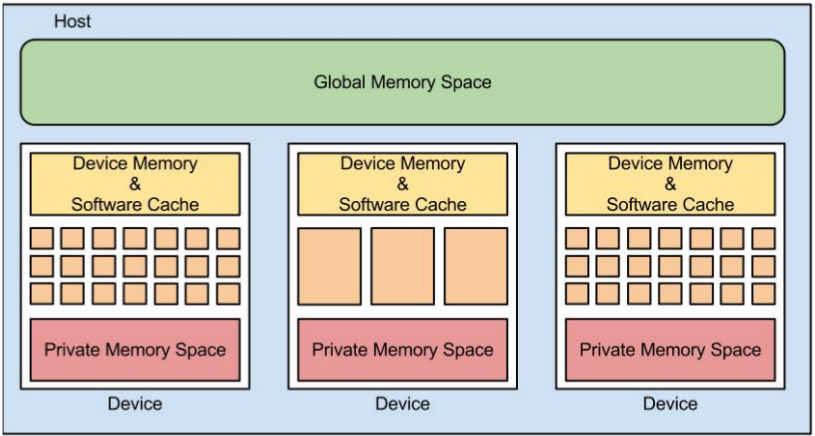
\includegraphics[width=0.6\columnwidth]{UPEM.png}
  \caption{GAMA Memory and Execution Model}
  \label{fig:upem}
\end{figure}

\Cref{fig:upem} provides an overview of the memory model employed in GAMA. It is based on a hierarchy, composed of three levels:
\begin{itemize}
  \item The first level is private and refers to a memory space addressable only by a single task
  \item The second level is shared between all Computational Units of a single device, and thus can be shared across tasks that are running on the same device. It is not addressable by other devices, however.
  \item Finally, the global level is addressable by the entire host system. However, due to implementation details of atomic operations being undefined, this level uses a relaxed consistency model, and requires explicit synchronization barriers to be used in order to ensure data consistency. 
\end{itemize}

Besides the memory hierarchy, GAMA also employs a software cache to reduce latency in global memory space accesses and to exploit potential temporal and spatial locality. This cache is typically implemented over the private memory address space of each device, and can also operate as a pre-fetch mechanism, as it has the ability of copying memory blocks to the device in which they are required, prior to the execution of the corresponding task.

